\section{Measurement}
\label{section:measurement}

\subsection{\bf Experiment Setup}

Fill experiment setup here.

\subsection{\bf Workload Description}
We have run three different kinds of workloads: read, write, and replication level change. For read, we have four clients each read 1 GB of data in ...

TODO: fill here.

\subsection{\bf Flow Size Analysis}
We have analyzed the flow size for each specific type of flows, and the results are shown in figure \ref{fig:read_size}, \ref{fig:write_size} and \ref{fig:replica_size}.

%\begin{figure*}[htb]
\begin{figure*}[!ht]
\label{fig:read_size}
\centering	
    \begin{tabular}{@{}cc@{}}
	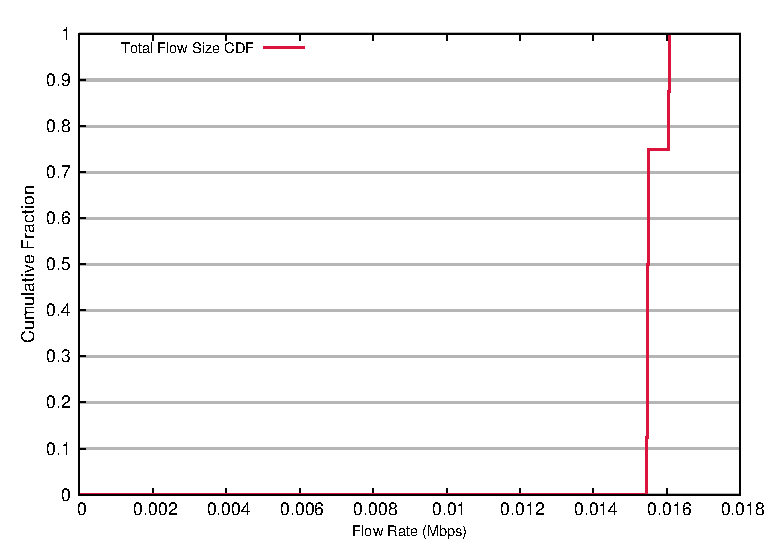
\includegraphics[width=.55\textwidth]{figures/4read/24_28_flow_size.eps} &
	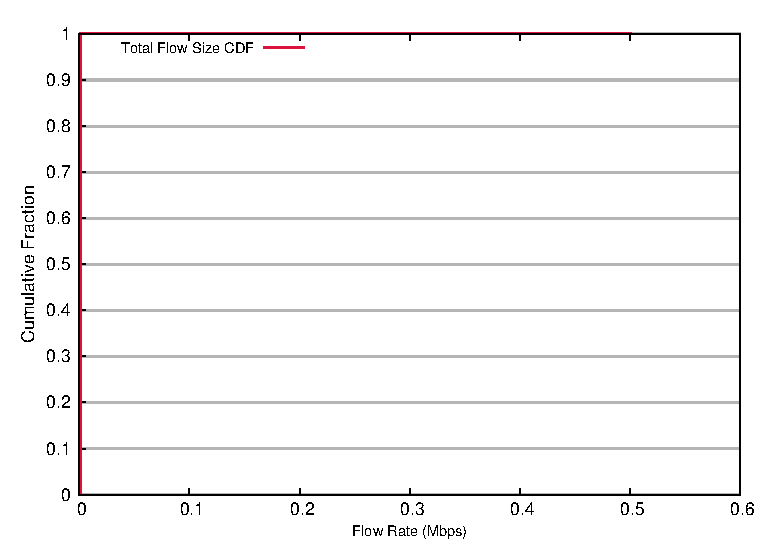
\includegraphics[width=.55\textwidth]{figures/4read/8_12_flow_size.eps}  \\
	\multicolumn{2}{c}{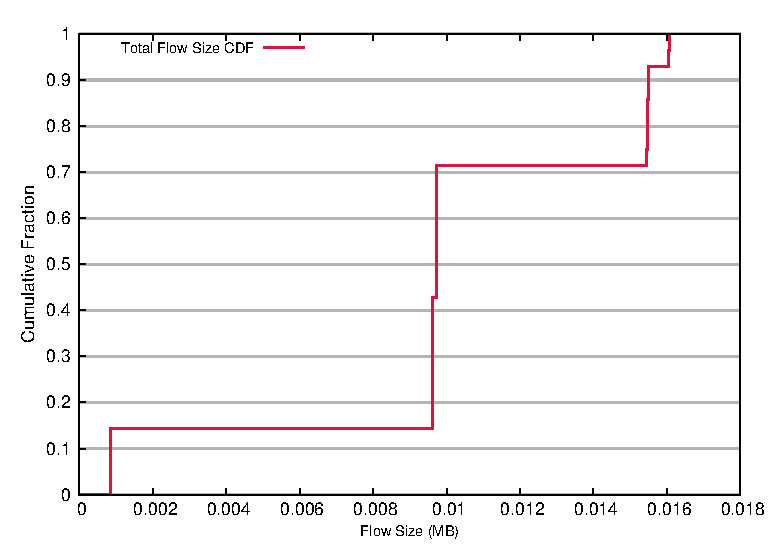
\includegraphics[width=.73\textwidth]{figures/4read/flow_size.eps}}
     \end{tabular}
\caption{Read Flow Size Distribution}
\end{figure*}

\begin{figure*}[!ht]
\label{fig:read_size}
\centering
  \begin{subfigure}[b]{.45\linewidth}
   \centering
	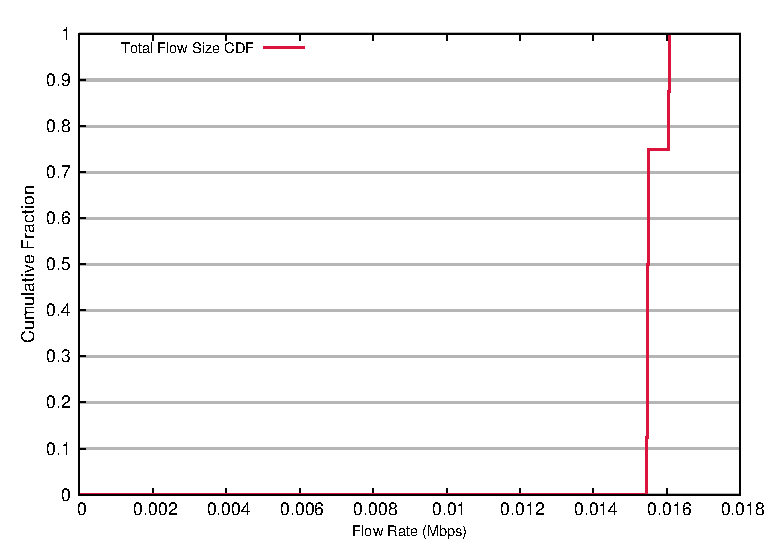
\includegraphics[width=.99\textwidth]{figures/4read/24_28_flow_size.eps} 
	\caption{RPC between Client and DataNodes}\label{fig:read_size:rpc}
   \end{subfigure}%
  \begin{subfigure}[b]{.45\linewidth}
   \centering
	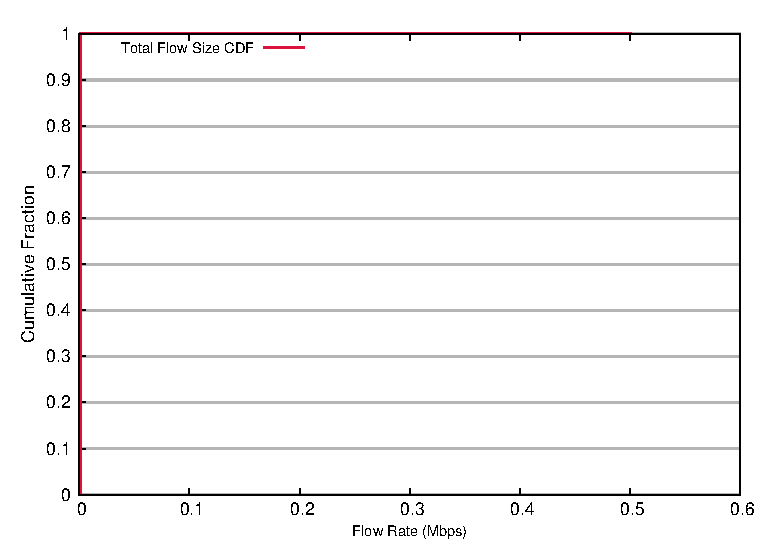
\includegraphics[width=.99\textwidth]{figures/4read/8_12_flow_size.eps} 
	\caption{Should have read data transfer here}\label{fig:read_size:fixme}
   \end{subfigure} \\%
  \begin{subfigure}[b]{.75\linewidth}
   \centering
	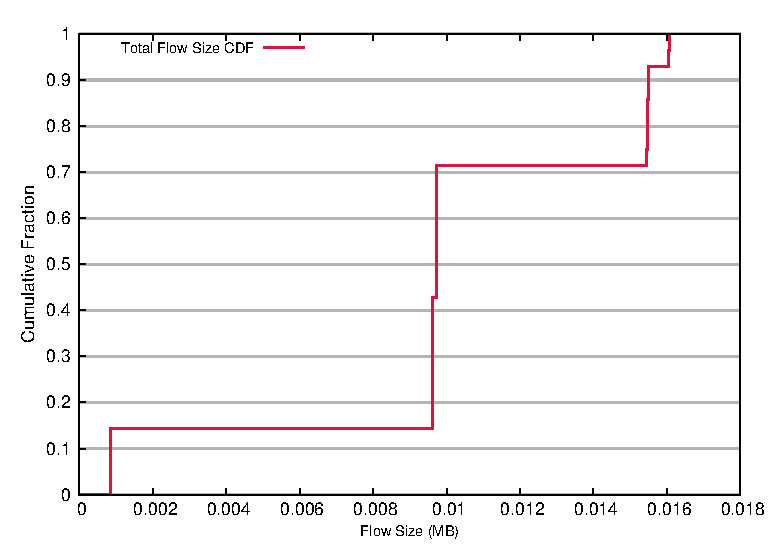
\includegraphics[width=.99\textwidth]{figures/4read/flow_size.eps}
	\caption{All Traffic}\label{fig:read_size:all}
   \end{subfigure}%
\caption{Read Flow Size Distribution}
\end{figure*}

\begin{figure*}[!ht]
\label{fig:write_size}
\centering
  \begin{subfigure}[b]{.45\linewidth}
   \centering
	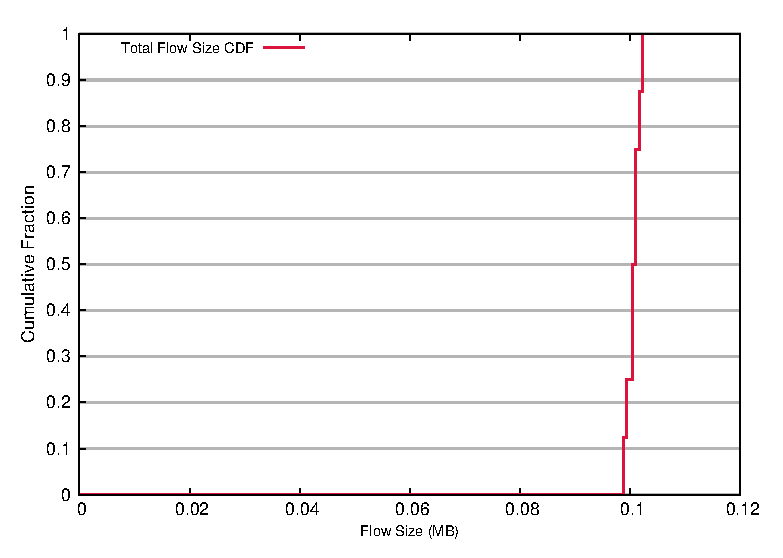
\includegraphics[width=.99\textwidth]{figures/6writes/24_28_type_flow_size.eps} 
	\caption{DataNodes RPC with NameNode}\label{fig:write_size:dn_rpc}
   \end{subfigure}%
  \begin{subfigure}[b]{.45\linewidth}
   \centering
	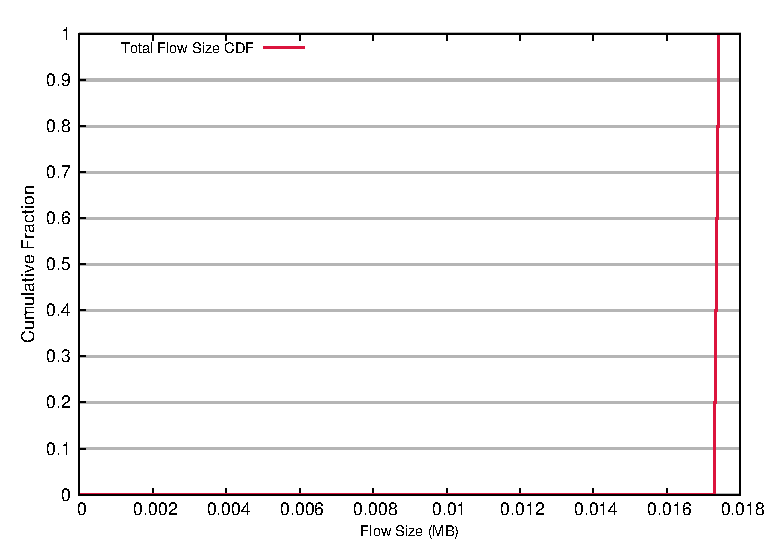
\includegraphics[width=.99\textwidth]{figures/6writes/24_28_20_16_type_flow_size.eps} 
	\caption{Client and DataNodes RPC with NameNode}\label{fig:write_size:dc_rpc}
   \end{subfigure} \\%
  \begin{subfigure}[b]{.45\linewidth}
   \centering
	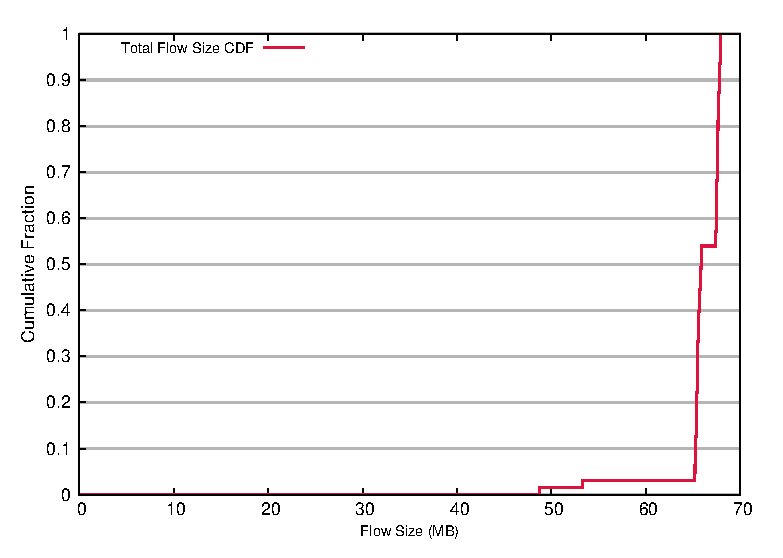
\includegraphics[width=.99\textwidth]{figures/6writes/36_44_type_flow_size.eps} 
	\caption{Pipelined Writes between DataNodes}\label{fig:write_size:pipe_write}
   \end{subfigure} %
  \begin{subfigure}[b]{.45\linewidth}
   \centering
	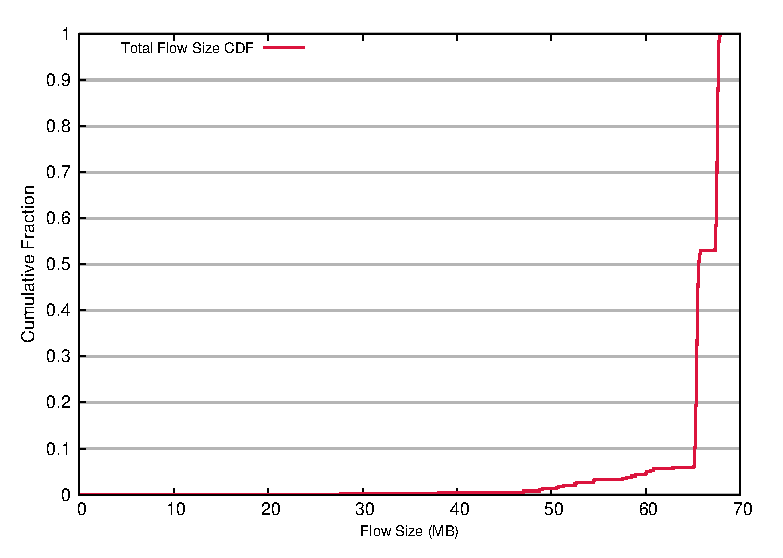
\includegraphics[width=.99\textwidth]{figures/6writes/32_36_type_flow_size.eps} 
	\caption{Client Data Transfer to DataNodes}\label{fig:write_size:client_write}
   \end{subfigure} \\%
  \begin{subfigure}[b]{.75\linewidth}
   \centering
	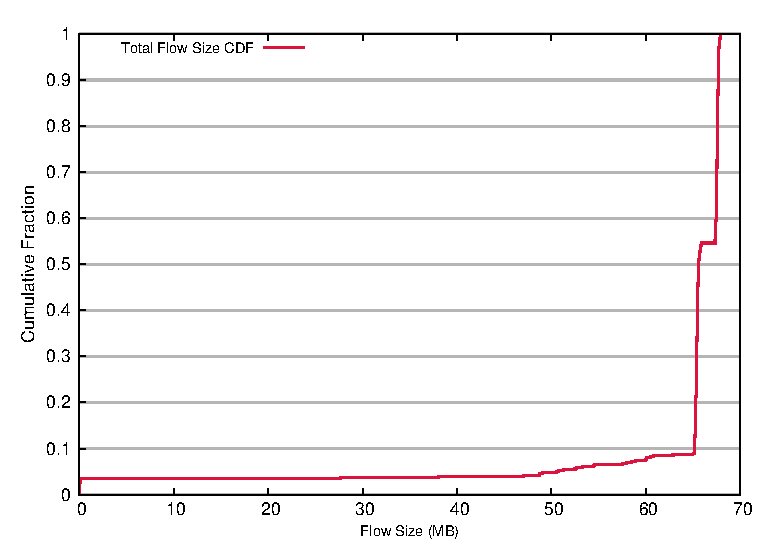
\includegraphics[width=.99\textwidth]{figures/6writes/flow_size.eps}
	\caption{All Traffic}\label{fig:write_size:all}
   \end{subfigure}%
\caption{Write Flow Size Distribution}
\end{figure*}

\begin{figure*}[!ht]
\label{fig:replica_size}
\centering
  \begin{subfigure}[b]{.45\linewidth}
   \centering
	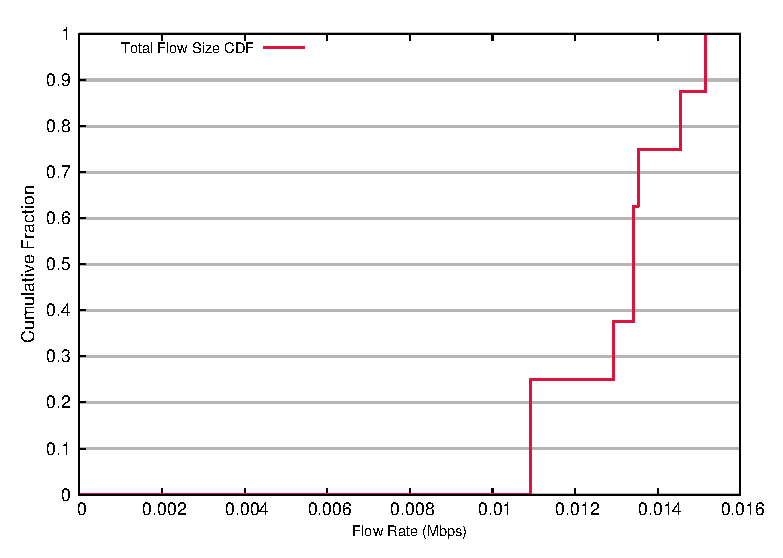
\includegraphics[width=.99\textwidth]{figures/replica_change/24_28_flow_size.eps} 
	\caption{DataNodes RPC with NameNode}\label{fig:replica_size:rpc}
   \end{subfigure}%
  \begin{subfigure}[b]{.45\linewidth}
   \centering
	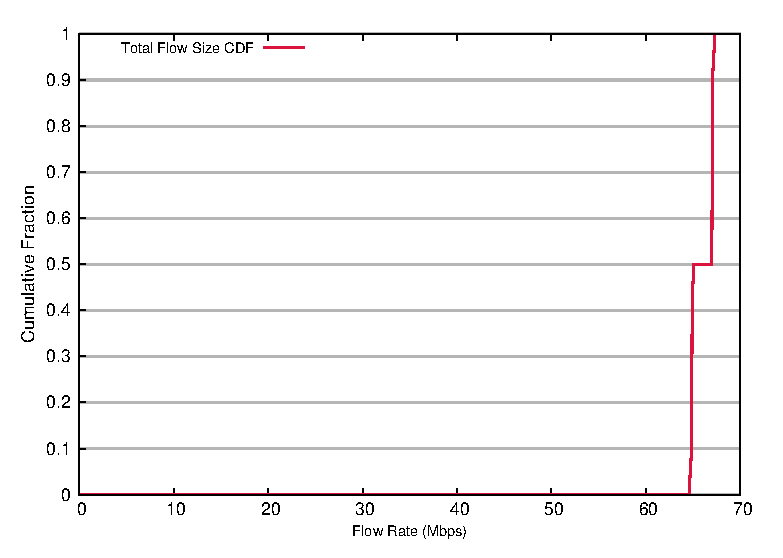
\includegraphics[width=.99\textwidth]{figures/replica_change/36_32_flow_size.eps} 
	\caption{Pipelined Writes between DataNodes}\label{fig:replica_size:pipe_write}
   \end{subfigure} \\%
  \begin{subfigure}[b]{.75\linewidth}
   \centering
	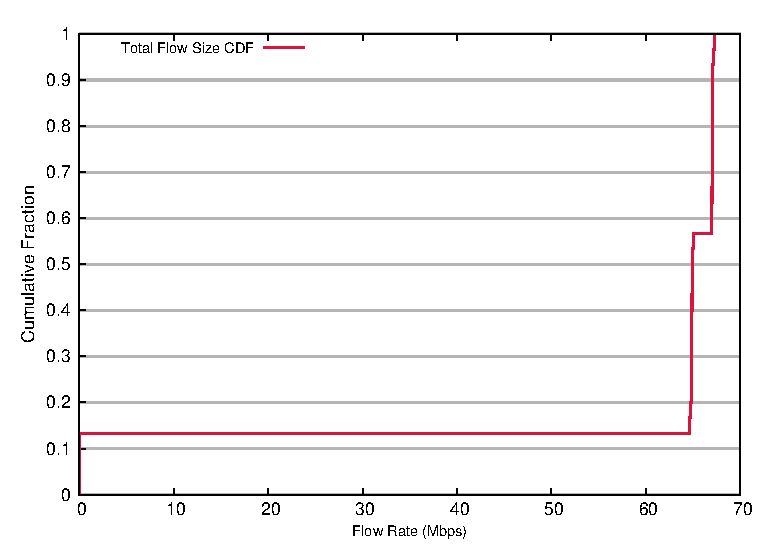
\includegraphics[width=.99\textwidth]{figures/replica_change/flow_size.eps}
	\caption{All Traffic}\label{fig:read_size:all}
   \end{subfigure}%
\caption{Replciation Level Change Flow Size Distribution}
\end{figure*}

